
\documentclass[12pt]{article}

\usepackage[margin=1in]{geometry}

% For vertical brace rcases
\usepackage{mathtools}
% For positioning figures
\usepackage{float}
% makes figure font bold
\usepackage{caption}
\captionsetup[figure]{labelfont=bf}
% For text generation
\usepackage{lipsum}
% For drawing
\usepackage{tikz}
% For manipulating coordinates
\usetikzlibrary{calc}
% For smaller or equal sign and not divide sign
\usepackage{amssymb}
% For the diagonal fraction
\usepackage{xfrac}
% For enumerating exercise parts with letters instead of numbers
\usepackage{enumitem}
% For dfrac, which forces the fraction to be in display mode (large) e
% even in math mode (small)
\usepackage{amsmath}
% For degree sign
\usepackage{gensymb}
% For "\mathbb" macro
\usepackage{amsfonts}
\newcommand{\N}{\mathbb{N}}
\newcommand{\Z}{\mathbb{Z}}
\newcommand{\Q}{\mathbb{Q}}
\newcommand{\R}{\mathbb{R}}
\newcommand{\C}{\mathbb{C}}
\newcommand{\F}{\mathbb{F}}
\newcommand{\rad}{\text{ rad}}

% overline short italic
\newcommand{\olsi}[1]{\,\overline{\!{#1}}}

\title{%
    \Huge Abstract Algebra \\
    \large by \\
    \Large Dummit and Foote \\~\\
    \huge Part 1: Group Theory \\
    \LARGE Chapter 1: Introduction to Groups \\
    \Large Section 6: Homomorphisms and Isomorphisms
}
\date{2023-07-14}
\author{Michael Saba}

\begin{document}
    \pagenumbering{gobble}
    \maketitle
    \newpage
    \pagenumbering{arabic}


    \section*{Exercise 1 $***$}
    For two groups $G$ and $H$,
    we condier the homomorphism $\varphi: G \to H$. \\ 
    \begin{enumerate}[label=\textbf{\alph*.}]
        \item 
            Proof that $\varphi(x^n) = \varphi(x)^n$ $\forall x \in G$
            and $n \in \Z^+$: \\
            Knowing that $\varphi$ is a homomorphism,
            we can use induction to prove the statement: \\
            \textbf{Basis step:}
            For $n = 2$,
            by the definition of a homomorphism,
            $\varphi(ab) = \varphi(a)\varphi(b)$.
            So $\varphi(x^2) = \varphi(xx)
            = \varphi(x)\varphi(x)
            = \varphi(x)^2$. \\
            \textbf{Inductive hypothesis:}
            Assume that for $n = k$, $\varphi(x^k) = \varphi(x)^k$. \\ 
            \textbf{Inductive step:}
            For $n = k+1$,
            we assumed that $\varphi(x^k) = \varphi(x)^k$,
            so $\varphi(x^{k+1}) = \varphi(x^kx)
            = \varphi(x^k)\varphi(x)
            = \varphi(x)^k\varphi(x)
            = \varphi(x)^{k+1}$.
            This completes the proof.
        \item
            Proof that $\varphi(x^{-1}) = \varphi(x)^{-1}$
            $\forall x \in G$: \\
            We know that $\varphi(ab) = \varphi(a)\varphi(b)$,
            and we also know that $\varphi(1_G) = 1_H$.
            So $\varphi(xx^-1) = \varphi(1_G) = 1_H$
            and $\varphi(xx^-1) = \varphi(x)\varphi(x^{-1})$.
            So $\varphi(x)\varphi(x^{-1}) = 1_H$,
            which implies that
            $\varphi(x)^{-1}\varphi(x)\varphi(x^{-1}) = \varphi(x)^{-1}$,
            which in turn tells us that
            $\varphi(x^{-1}) = \varphi(x)^{-1}$
            (since $\varphi$ is well defined). \\
            From the two statements we have proved,
            we conclude that by setting $y = x^n$ for $n \in \Z^+$,
            $ \varphi(x^{-n}) = \varphi((x^n)^{-1})
            = \varphi(y^{-1})
            = \varphi(y)^{-1}
            = \varphi(x^n)^{-1}
            = (\varphi(x)^n)^{-1}
            = \varphi(x)^{-n}$.
            Since we've shown the proposition in part a applies for $n < 0$,
            and since $\varphi(1_G) = 1_H$ implies it works for
            $n = 0$, we conclude that $\forall n \in \Z$, 
            $\varphi(x^n) = \varphi(x)^n$.
    \end{enumerate}


    \section*{Exercise 2 $***$}
    For two groups $G$ and $H$,
    we condier the isomorphism $\varphi: G \to H$. \\ 
    Proof that $\forall x \in G$, $|x| = |\varphi(x)|$: \\
    Assume that $\exists x \in G$
    such that  $|x| \neq |\varphi(x)|$.
    Since $\varphi$ is bijective,
    then $\varphi(a) = \varphi(b)$ if and only if $a = b$.
    Now, let us take $n = |x|$ and $m = |\varphi(x)|$
    and consider the following cases:
    \begin{enumerate}[label=\textbf{case \arabic*:}]
        \item
            If $m < n < \infty$,
            then $|x| > |\varphi(x)|$.
            then as $|x| = n$,
            $n$ is the smallest power to which $x$ becomes the identity.
            Since $m < n$, $x^m \neq 1_G$.
            Since $\varphi$ is bijective,
            and $\varphi(1_G) = 1_H$,
            $\varphi(x^m) \neq 1_H$.
            But we know that $|\varphi(x)| = m$,
            so $\varphi(x)^m = 1_H$.
            This implies that $\varphi(x^m) \neq \varphi(x)^m$,
            which contradicts the proposition we proved in exercise 1.1.6.1.
        \item 
            If $n < m < \infty$,
            then $|x| < |\varphi(x)|$.
            then as $|\varphi(x)| = m$,
            $m$ is the smallest power to which $\varphi(x)$ becomes the
            identity.
            Since $m > n$, $\varphi(x)^n \neq 1_H$.
            We know that since $|x| = n$, $x^n = 1_G$,
            so $\varphi(x^n) = \varphi(1_G) = 1_H$. 
            Since $\varphi$ is bijective,
            $\varphi(x)^n \neq \varphi(x^n)$.
            which contradicts the proposition we proved in exercise 1.1.6.1.
        \item
            If $n = \infty$ and $m < \infty$,
            then $|x| > |\varphi(x)|$.
            then $x^m \neq 1_G$ as $x$ has infinite order.
            Since $\varphi$ is bijective,
            and $\varphi(1_G) = 1_H$,
            $\varphi(x^m) \neq 1_H$.
            But we know that $|\varphi(x)| = m$,
            so $\varphi(x)^m = 1_H$.
            This implies that $\varphi(x^m) \neq \varphi(x)^m$,
            which contradicts the proposition we proved in exercise 1.1.6.1.
        \item
            If $n < \infty$ and $m = \infty$,
            then $|x| < |\varphi(x)|$.
            then $\varphi(x)^n \neq 1_H$
            since $\varphi(x)$ has infinite order.
            We know that since $|x| = n$, $x^n = 1_G$,
            so $\varphi(x^n) = \varphi(1_G) = 1_H$. 
            Since $\varphi$ is bijective,
            $\varphi(x)^n \neq \varphi(x^n)$.
            which contradicts the proposition we proved in exercise 1.1.6.1.
    \end{enumerate}   
    Since each case led to a contradiction,
    we conclude that $\forall x \in G$, $|x| = |\varphi(x)|$. \\
    Since isomorphisms are bijective by nature,
    if they map two groups together,
    the two groups must have the same order.
    This fact, coupled with the statement we just proved,
    tells us that for any fixed $n \in \Z^+$,
    there are the same number of elements of order $n$ the two groups. \\
    The statement we proved doesn't necessarily stand
    if $\varphi$ were a homomorphism.
    This is because in our proof, we utilize the fact that
    $\varphi(a) = \varphi(b)$ implies that $a = b$ in a bijection,
    which need not be the case with a homomorphism.
    To show that there are instances when this isn't the case,
    we can give a counterexample. \\
    Take $\phi: G \to H$ where $\phi$ is a homomorphism,
    $H$ is the trivial group $\{1\}$, $G$ is not,
    and $\phi(a) = 1_H$ $\forall a \in G$.
    This is clearly a homomorphism
    as $\phi(ab) = 1_H = 1_H1_H = \phi(a)\phi(b)$.
    But since $G$ is not the trivial group,
    then some element with an order larger than 1 will be mapped to $1_H$,
    demonstrating our example.


    \section*{Exercise 3 $***$}
    For two groups $G$ and $H$, we condier the isomorphism $\varphi: G \to H$.
    Proof that $G$ is abelian if and only if $H$ is abelian: \\
    If $G$ is abelian,
    then $\forall a, b \in G$, $ab = ba$.
    So $\varphi(ab) = \varphi(a)\varphi(b)
    = \varphi(ba)
    = \varphi(b)\varphi(a)$.
    Since $\varphi$ is surjective (since it's bijective),
    every element $c \in H$ is the image of some element in $G$.
    So $\varphi(a)\varphi(b) = \varphi(b)\varphi(a)$
    implies that all elements of $H$ commute,
    as all can be written as the image of some element of $G$. \\
    Converesely, if $H$ is abelian, 
    then $\forall c, d \in H$, $cd = dc$.
    Since $\varphi$ is bijective,
    there exists a two sided inverse $\varphi^{-1}: H \to G$,
    which is an isomorphism.
    We can easily show this,
    since $\varphi(ab) = \varphi(a)\varphi(b)$
    implies $\varphi^{-1}(\varphi(ab)) = \varphi^{-1}(\varphi(a)\varphi(b))$,
    which tells us $\varphi^{-1}$ is an isomorphism
    since $\varphi^{-1}(\varphi(a)) = a$,
    and $\varphi^{-1}(\varphi(b)) = b$.
    Since $\varphi^{-1}$ is an isomorphism and a bijection,
    we can apply the same proof we did before, proving the converse. \\
    Now, if $\varphi^{-1}$ were a homomorphism,
    we would need for it to also be surjective before the statement
    $G$ is abelian $\implies$ $H$ is abelian becomes true,
    since otherwise, elements in $H$ could be immune to the structural
    constraints the homomorphism places on $H$.
    Note that surjection alone is not enough to prove that 
    $G$ is abelian $\iff$ $H$ is abelian,
    as the converse requires a full bijection (in the proof). 


    \section*{Exercise 4 $***$}
    Proof that the multiplicative groups $G = (\R - \{0\}, \times)$
    and $H = (\C - \{0\}, \times)$ are not isomorphic: \\
    In exercise 1.1.6.2 we showed that two isomorphic groups contain the same
    number of elements with order $n$ for any $n \in \Z^+$.
    In $G$, we have only one element of order 3.
    This is because 1 is the multiplicative identity of $G$,
    and $x^3 = 1$ only has a solution at $x = 1$ in $\R$. \\
    However, in $H$, the equation $x^3 = 1$ has 3 solutions:
    \[x_1 = 1, \text{ } x_2 = \dfrac{-1 + i\sqrt{3}}{2}
    \text{ and } x_3 = \dfrac{-1 - i\sqrt{3}}{2}\]
    So 3 elements in $H$ have order 3,
    which contradicts the property we proved in exercise 1.1.6.2.
    Thus $G$ and $H$ are not isomorphic. 
    

    \section*{Exercise 5}
    Proof that the multiplicative groups $(\R, +)$
    and $(\C, +)$ are not isomorphic: \\
    While both groups are of infinite order,$
    \R$ is a larger type of infinity than $\Q$.
    $\R$'s infinity is called uncountable and denoted $2^{\aleph_0}$.
    $\Q$'s infinity is called countable and denoted $\aleph_0$.
    By definition, one infinity beling larger than another means that
    we can't have a 1 to 1 mapping between the two.
    Since there exists no bijections between $\R$ and $\Q$,
    they can't be isomorphic.


    \section*{Exercise 6 $***$}
    Proof the additive groups $\Z$ and $\Q$ are not isomorphic: \\
    Suppose that $\phi: \Q \to \Z$ is an isomorphism.
    Then there must exist an element $q \in \Q$
    such that $\phi(q) = 1_\Z$.
    We know frome exercise 1.1.6.1 that in an isomorphism,
    $\phi(n \cdot x) = n \cdot \phi(x)$ $\forall x \in \Q$,
    (but with addition rather than multiplication as the group operation).
    So $\phi(q) = \phi(2(\sfrac{q}{2})) = 2\phi(q/2) = 1_\Z = 1$.
    So $1 = 2\phi(\sfrac{q}{2})$, meaning $\phi(\sfrac{q}{2}) = \sfrac{1}{2}$.
    But since $\sfrac{1}{2} \notin \Z$,
    then $\sfrac{q}{2}$ does not have an image,
    meaning $\phi$ is not a function, which is a contradiction.
    So the groups $(\Z, +)$ and $(\Q, +)$ are not isomorphic.


    \section*{Exercise 7}
    Proof that $D_8$ and $Q_8$ are not isomorphic: \\
    In $Q_8$, we only have one element with order 2 ($-1$).
    In $D_8$ however, both $r^2$, $s$, and others have order 2.
    This contradicts our findinsg in exercise 1.1.6.2,
    so $Q_8$ and $D_8$ are not isomorphic.


    \section*{Exercise 8}
    Proof that if $n \neq m$, then $S_n \ncong S_m$: \\
    If two groups are isomorphic,
    then there exists a bijection from the first to the second.
    That means that they must both have the same order.
    If $n \neq m$, and both are finite,
    then $|S_n| = n! \neq |S_m| = m!$. 
    On the other hand, if one of the two were infinite,
    then one of the groups would have a finite order and the other an
    infinite order.
    Either way, $|S_n| \neq |S_m|$,
    so they can't be isomorphic.


    \section*{Exercise 9}
    Proof that $D_{24} \ncong S_4$: \\
    In $D_{24}$, $r$ has order 12.
    But in $S_4$, the possible disjoint cycle permutation sizes are:
    $lcm(4) = 4$, $lcm(3) = 3$, $lcm(2, 2) = 2$, $lcm(2) = 2$.
    So there doesn't exist any elements in $S_4$ with order 12.
    So by the statement we proved in exercise 1.1.6.2,
    $D_{24}$ and $S_4$ can't be isomorphic.


    \section*{Exercise 10 $***$}
    Proof that $S_\triangle \cong S_\Omega$
    if $|\triangle| = |\Omega|$: \\
    Consider the bijective map $\theta: \triangle \to \Omega$
    (possible since both sets have the same order).
    As $\theta$ is a bijection between two sets,
    we can consider it to be a permutation of the elements in $\triangle$. \\
    Now consider the map $\varphi: S_\triangle \to S_\Omega$
    where $\forall \sigma \in S_\triangle$,
    $\varphi(\sigma) = \theta \circ \sigma \circ \theta^{-1}$
    (where $\theta^{-1}$ is the inverse map of $\theta$,
    meaning that it bijectively maps $\Omega$ to $\triangle$,
    making it another permutation): \\
    \begin{enumerate}[label=\textbf{\alph*.}]
        \item 
            Proof that $\varphi$ is well defined
            (meaning that the relation is a function, where each
            element in $S_\triangle$ has one and only one image): \\
            We have $\theta \circ \sigma \circ \theta^{-1}
            = \theta(\sigma(\theta^{-1}))$.
            Starting from the inside out,
            we know that $\theta^{-1}$ maps $\Omega$ to $\triangle$,
            then $\sigma$ maps $\triangle$ to itself (permutes it),
            and finally, $\theta$ maps $\triangle$ to $\Omega$.
            Since each of these maps is individually bijective,
            and since the composition of these maps maps $\Omega$
            to $\Omega$,
            that must mean that every element $\varphi(\sigma)$,
            is a permutation of $\Omega$,
            so  $\varphi(\sigma) \in \S_\Omega$.
            And as $\sigma$, $\theta$ and $\theta^{-1}$ are all bijective,
            then each $\sigma \in S_\triangle$ maps to only one value
            in $S_\Omega$,
            making $\varphi$ well defined.
        \item
            Proof that $\varphi$ is bijective: \\
            We can show that $\varphi$ is a bijection by finding a two-sided
            inverse.
            That means, we need to find a map
            $\varphi^{-1}: S_\Omega \to S_\triangle$
            such that $\varphi \circ \varphi^{-1}
            = \varphi^{-1} \circ \varphi$ is the identity map of 
            $S_\Omega$ and $S_\triangle$ respectively.
            Consider the map $\varphi^{-1}: S_\Omega \to S_\triangle$
            where $\varphi^{-1}(\tau)
            = \theta^{-1} \circ \tau \circ \theta$
            $\forall \tau \in S_\Omega$. \\
            We have $\varphi^{-1}(\varphi(\sigma))
            = \varphi^{-1}(\theta \circ \sigma \circ \theta^{-1})
            = \theta^{-1} \circ \theta \circ \sigma \circ \theta^{-1}
            \circ \theta
            = \sigma$ $\forall \sigma \in S_\triangle$. \\
            We also have $\varphi(\varphi^{-1}(\tau))
            = \varphi(\theta^{-1} \circ \tau \circ \theta)
            = \theta \circ \theta^{-1} \circ \tau \circ \theta
            \circ \theta^{-1}
            = \tau$ $\forall \tau \in S_\Omega$. \\
            So $\varphi^{-1}$ is a two-sided inverse,
            which means that $\varphi$ is bijective.
        \item
            Proof that $\varphi$ is a homomorphism: \\
            First, we note that since $\theta$ is bijective
            and $\theta^{-1}$ its inverse,
            that $\theta^{-1} \circ \theta$ is the identity map 1. \\
            Moreover, for all $\sigma, \tau \in S_\triangle$,
            we have $\varphi(\sigma \circ \tau)
            = \theta \circ \sigma \circ \tau \circ \theta^{-1}
            = \theta \circ \sigma \circ 1 \circ \tau \circ \theta^{-1}
            = \theta \circ \sigma \circ (\theta^{-1} \circ \theta) \circ \tau
            \circ \theta^{-1}
            = (\theta \circ \sigma \circ \theta^{-1}) \circ (\theta \circ
            \tau \circ \theta^{-1})
            = \varphi(\sigma) \circ \varphi(\tau)$.
            So $\varphi$ is a homomorphism and a bijection,
            which makes it an isomorphism.
    \end{enumerate}


    \section*{Exercise 11}
    Proof that if $A$ and $B$ are groups,
    then $A \times B \cong B \times A$: \\
    Consider the map $\phi: A \times B \to B \times A$
    where $\forall a\in A$ and $b \in B$, $\phi((a, b)) = (b, a)$. \\
    This is trivially well defined since we are only swapping the two tuples,
    which we know always map to a single element in their respective sets.
    Futhermore, we have $\phi((a, b)(c, d)) = \phi((ac, bd))
    = (bd, ac) = (b, a)(d, c) = \phi(a, b)\phi(c, d)$,
    so $\phi$ is a homomorphism.
    Furthermore, this is clearly a bijection,
    since $\forall (a, b) \in A \times B$,
    there exists exactly one element in $B \times A$
    such that the first tuple is $b$ and the second is $A$.
    So $\phi$ is an isomorphism,
    which means  $A \times B \cong B \times A$.


    \section*{Exercise 12}
    Proof that for grousp $A$, $B$, and $C$, if $G = A \times B$
    and $H = B \times C$, then $G \times C \cong A \times H$
    (the two groups $(A \times B) \times C$ and $A \times (B \times C)$
    aren't the same as the cartesian product is not associative): \\
    Consider the map $\phi: G \times C \to A \times H$
    where $\forall a \in A$, $\forall b \in B$, and $\forall c \in C$,
    $\phi(((a, b), c)) = (a, (b, c))$.
    This mapping is obviously well defined and bijective
    because for each $((a, b), c) \in G \times C$,
    there exists exactly one tuple in $A \times H$ with the elements
    $a$, $b$, and $c$. \\
    Moreover, $\phi$ is a homomorphism 
    since $\phi(((a, b), c)((d, e), f)) = \phi(((ad, be), cf))
    = (ad, (be, cf))
    = (a, (b, c))(d, (e, f))
    = \phi(((a, b), c))\phi(((d, e), f))$.
    So as $\phi$ is both bijective and a homomorphism,
    then $G \times C \cong A \times H$.


    \section*{Exercise 13 $***$}
    Proof that for groups $G$ and $H$,
    if $\varphi: G \to H$ is a homomorphism,
    then $\varphi(G)$ is a subgroup of $H$,
    where $\varphi(G)$ is $G$'s image in $H$: \\
    First, by definition, since $\varphi$ maps $G$ to $H$,
    then $\varphi(G) \subseteq H$. \\
    Moreover $\varphi(G) \neq \emptyset$,
    since $\varphi(1_G) = 1_H$ belongs in $\varphi(G)$. \\
    Furthermore, $\varphi: G \to \varphi(G)$ is by definition surjective
    (it only contains the elements mapped from $G$).
    So $\forall a \in \varphi(G)$, $a = \varphi(g_a)$ where $g_a \in G$.
    Hence, $\forall a, b \in \varphi(G)$,
    $ab = \varphi(g_a)\varphi(g_b) = \varphi(g_ag_b)$
    where $g_ag_b \in G$,
    so $\varphi(g_ag_b) \in \varphi(G)$.
    And $\forall a \in \varphi(G)$,
    $a^{-1} = \varphi(g_a)^{-1} = \varphi(g_a^{-1})$
    where $g_a^{-1} \in G$,
    so $\varphi(g_a^{-1}) \in \varphi(G)$. \\
    Thus $\varphi(G)$ is closded under multiplication and inverses,
    and is a non-empty subset of $H$,
    so $\varphi(G) \leqslant H$. \\
    Proof that if $\varphi$ is injective, then $G \cong \varphi(G)$: \\
    We showed that by definition, $\varphi$ is surjective.
    So if it is also injective, that would make it a bijection.
    Since $\varphi$ is a homomorphism relationship by assumption,
    then $G$ and $\varphi(G)$ are isomorphic.


    \section*{Exercise 14 $***$}
    Proof that if the map $\varphi: G \to H$ is a homomorphism,
    then the kernel of the the homomorphism $\varphi$ defined as the set
    $\{g \in G \mid \varphi(g) = 1_H\}$ (also known as the
    \textit{fiber over the identity of $H$})
    and denoted by $\ker \varphi$ is a subgroup of $G$: \\
    As we know $\varphi(1_G) = 1_H$, so $1_G \in \ker \varphi$,
    which means that $\ker \varphi \neq \emptyset$.
    Moreover, since $\ker \varphi = \{g \in G \mid \varphi(g) = 1_H\}$,
    then it's trivially a subset of $G$.
    Furthermore, if $a, b \in \ker \varphi$,
    then for $ab \in G$,
    we have $\varphi(ab) = \varphi(a)\varphi(b) = 1_H1_H = 1_H$,
    so $ab \in \ker \varphi$.
    And for $a^{-1} \in G$,
    we have $\varphi(a^{-1}) = \varphi(a)^{-1} = 1_H^{-1} = 1_H$,
    so $a^{-1} \in \ker \varphi$.
    So the kernel is closed under inverses and the group action,
    and is also a non-empty subset of $G$,
    which means that $\ker \varphi \leqslant G$. \\
    Proof that $\varphi$ is injective if and only if
    $\ker \varphi$ is the identity subgroup $\{1_G\}$ of $G$: \\
    First, assume that $\ker \varphi = \{1_G\}$.
    This means that $1_G$ is the only element in $G$ that maps to $1_H$.
    This means that $\varphi$ is injective,
    and we can prove that by contradiction: \\
    Assume that there exists two elements $a, b \in G$
    such that $a \neq b$ but $\varphi(a) = \varphi(b)$.
    So $\varphi(ab^{-1}) = \varphi(a)\varphi(b^{-1})
    = \varphi(b)\varphi(b)^{-1} = 1_H$.
    Since inverses are unique in groups, $a^{-1} \neq b^{-1}$,
    so $ab^{-1} \neq 1_H$, but $\varphi(ab^{-1}) = 1_H$,
    which contradicts our assumption,
    proving that if $a \neq b$, $\varphi(a) \neq \varphi(b)$
    for all elements in $G$,
    making $\varphi$ injective. \\ 
    Conversely, if $\varphi$ is injective,
    then by definition only one element can map to $1_H$.
    We know that since $\varphi$ is a homomorphism,
    then $\varphi(1_G) = \varphi(1_H)$,
    so $1_G$ is the only element that maps to $1_H$,
    which means that $\ker \varphi = \{1_G\}$. 


    \section*{Exercise 15}
    Proof that the map $\pi: \R^2 \to \R$,
    where $\pi((x, y)) = x \forall x, y \in \R$, is an homomorphism: \\
    This map is well defined because for each tuple in $\R^2$
    unambiguously maps to exactly one element in $\R$
    since it's the first element in the tuple itself.
    Moreover, $\forall (x, y), (z, w) \in \R^2$,
    $\pi((x, y)(z, w)) = \pi((xz, yw)) = xz = \pi((x, y))\pi((z, w))$,
    so $\pi$ is a homomorphism. \\
    Additionally, $\ker \pi$ is the set of elements that map to $0$
    (the additive identity of $\R$),
    so $\ker \pi = \{(0, r) \mid r \in \R\}$.                                                       


    \section*{Exercise 16}
    Proof that if $A$ and $B$ are groups and $G = A \times B$,
    then the maps $\pi_1: G \to A$ and $\pi_2: G \to B$ defined by
    $\pi_1((a, b)) = a$ and $\pi_2((a, b)) = b$ are homomorphisms: \\
    Using the same argument we used in exercise 1.1.6.15,
    we can show that $\pi_1$ and $\pi_2$ are well defined
    (this is because for each tuple, there is exactly one umabiguous image,
    seeing as the image is one of the elements in the tuple).\\
    Moreover, we have, $\forall (a, b), (c, d) \in G$,
    \[ \pi_1((a, b)(c, d)) = \pi_1((ac, bd))
    = ac
    = \pi_1((a, b))\pi_1((c, d)) \]
    and
    \[ \pi_2((a, b)(c, d)) = \pi_2((ac, bd))
    = bd
    = \pi_2((a, b))\pi_2((c, d)) \]
    So both $\pi_1$ and $\pi_2$ are homomorphisms. \\
    Furthermore, we have $\ker \pi_1 = \{(1_A, b) \mid b \in B\}$
    and $\ker \pi_2 = \{(a, 1_B) \mid a \in A\}$.


    \section*{Exercise 17}
    Proof that for a group $G$, $\varphi: G \to G$
    defined by $\varphi(g) = g^{-1}$ $\forall g \in G$
    is a homomorphism if and only if $G$ is abelian: \\
    The map is well defined as a result of the inverse's uniqueness. \\
    First, assume that $G$ is abelian.
    In that case, $\forall a, b \in G$,
    $\varphi(ab) = (ab)^{-1} = b^{-1}a^{-1} 
    = a^{-1}b^{-1}
    = \varphi(a)\varphi(b)$.
    This makes $\varphi$ a homomorphism. \\
    Converesely, if $\varphi$ is a homomorphism,
    then $\varphi(ab) = (ab)^{-1}
    = \varphi(a)\varphi(b)
    = a^{-1}b^{-1} 
    = (ba)^{-1}$.
    That $(ab)^{-1} = (ba)^{-1}$ implies that $ab = ba$ $\forall a, b \in G$.
    So $G$ is abelian.


    \section*{Exercise 18}
    Proof that for a group $G$, $\varphi: G \to G$
    defined by $\varphi(g) = g^2$ $\forall g \in G$
    is a homomorphism if and only if $G$ is abelian: \\
    The map is well defined since for each $x \in G$, since $x^2$ is unique
    and unambiguous and $G$ is closed under the group operation. \\
    First, assume that $G$ is abelian.
    In that case, $\forall a, b \in G$,
    $\varphi(ab) = (ab)^2
    = abab
    = aabb
    = a^2b^2
    = \varphi(a)\varphi(b)$.
    This makes $\varphi$ a homomorphism. \\ 
    Converesely, if $\varphi$ is a homomorphism,
    then $\varphi(ab) = (ab)^{2}
    = abab
    = \varphi(a)\varphi(b)
    = a^{2}b^{2} 
    = aabb$.
    So $abab = aabb$,
    which implies that $ab = ba$ $\forall a, b \in G$.
    So $G$ is abelian.
    

    \section*{Exercise 19}
    Let $G = \{z \in \C \mid z^n = 1 \text{ for some } n \in \Z^+ \}$
    be a multiplicative group with identity 1.
    Proof that for a fixed integer $k > 1$,
    the map $\varphi: G \to G$,
    defined by $\varphi(z) = z^k$ $\forall z \in G$,
    is a surjective homomorphism, but not an isomorphism: \\
    The map $\varphi$ is well defined since $z^k$ is unique
    and unambiguous and $G$ is closed under the group operation. \\
    Futhermore, $\forall x, y \in G$,
    $\varphi(xy) = (xy)^k = x^ky^k = \varphi(x)\varphi(y)$
    since multiplication is commutative in $\C$. 
    So $\varphi$ is a homomorphism. \\
    Additionally, $\forall z \in G$, $\exists n \in \Z^+$
    such that $z^n = 1$.
    So $z^{\sfrac{1}{k}}$, $(z^{\sfrac{1}{k}})^{nk} = (z^1)^{n} = 1$,
    which means that $\forall z \in G$, $z^{\sfrac{1}{k}} \in G$.
    So each element $z$ in $G$ is the image of an element in the input,
    which makes $\varphi$ surjective. \\
    The map is not an isomorphism however, as it is not injective.
    To show this, we first note that $1 = e^{2 \pi i}$,
    so $\forall n \in \Z$, $1 = e^{2 \pi i} = (e^{\sfrac{2 \pi i}{n}})^n$.
    Hence, all elements $e^{\sfrac{2 \pi i}{n}} \in G$.
    So for any fixed integer $k$ that is larger than 1,
    if we set $n = k$,
    we have $\varphi(e^{\sfrac{2 \pi i}{k}}) = e^{\sfrac{2k \pi i}{k}}
    = e^{2 \pi i} = 1$,
    and $\varphi(1) = 1^k = 1$.
    Since $k > 1$, $e^{\sfrac{2 \pi i}{k}} \neq 1$,
    so $\varphi$ is not injective,
    which means the groups are not isomorphic.
    

    \section*{Exercise 20 $***$}
    An automorphism is an isomorphism from a group to itself.
    Let $Aut(G)$ be the \textit{automorphism group of $G$},
    which is the set of all automorphisms of $G$ (set of functions).
    Proof that $Aut(G)$ is a group under function composition: \\
    An automorphism is a bijective mapping from $G$ to $G$.
    So for $\varphi, \phi \in Aut(G)$,
    $\varphi(\phi(ab)) = \varphi(\phi(a)\phi(b))
    = \varphi(\phi(a))\varphi(\phi(b))$,
    where $\varphi \circ \phi$ is a permutation (bijective mapping)
    and satisfies the constraints of a homomorphism, making it an
    isomorphism.
    So $Aut(G)$ is closed under composition. \\ 
    Moreover, if $A \cong B$, then $B \cong A$.
    This meand that for a bijection $\phi: G \to G$,
    $\phi^{-1}: G \to G$ is also a bijection.
    And if $\phi$ is an isomorphism,
    and $c = \phi^{-1}(a)$ and $d = \phi^{-1}(b)$,
    then $\phi^{-1}(ab) = \phi^{-1}(\phi(c)\phi(d))
    = \phi^{-1}(\phi(cd))
    = cd
    = \phi^{-1}(a)\phi^{-1}(b)$.
    So $\phi^{-1}$ is a bijection and a homomorphism, 
    making it an isomorphism,
    which means that $\phi^{-1} \in Aut(G)$ $\forall \phi \in Aut(G)$,
    so $Aut(G)$ is closed under inverses. \\
    Furthermore, since the identity function $I$ is obviously in $Aut(G)$,
    since it is trivially bijective
    and $I(ab) = ab = I(a)I(b)$.
    It's the identity of $Aut(G)$
    since $I \circ \phi = \phi \circ I = \phi$ $\forall \phi \in Aut(G)$. \\
    Finally, we know fucntion composition is by nature associative.
    So we conclude that $Aut(G)$ is a group under function composition.


    \section*{Exercise 21}
    Proof that for a fixed $k \in \Q - \{0\}$,
    the map $\phi : \Q \to \Q$ defined by $\phi(q) = kq$ $q \in \Q$ 
    (the additive group) is an automorphism: \\
    First, for $p, q \in \Q$,
    $\phi(p + q) = k(p + q) = kp + kq = \phi(p) + \phi(q)$,
    so $\phi$ is a homomorphism.
    Moreover, for every $q$ in $\Q$, $\sfrac{q}{k} \in \Q$
    since $k \neq 0$ and $\Q$ is closed under division.
    So every element $q$ in $\Q$ is the image of an element in $\Q$,
    making $\phi$ surjective.
    And as $|\Q| = |\Q|$, $\phi$'s surjectivity suggests it's injective,
    making the mapping a bijection,
    and by extension, an isomorphism,
    which in turn, makes it an automorphism.


    \section*{Exercise 22}
    Proof that for an abelian group $A$ and a fixed integer $k$,
    the mapping $\phi: A \to A$ defined by $\phi(a) = a^k$ $\forall a \in A$,
    is a homomorphism, and in the case of $k = -1$, an automorphism: \\
    First, for $a, b \in A$,
    since $A$ is abelian, then $a$ and $b$ commute,
    so by exercise 1.1.6.24 in section 1, $(ab)^k = a^kb^k$,
    so $\phi(ab) = (ab)^k = a^kb^k = \phi(a)\phi(b)$,
    so $\phi$ is a homomorphism. \\
    Now if $k = -1$,
    then $\forall a \in A$, $a^{-1} \in A$,
    and $\phi(a^{-1}) = (a^{-1})^{-1} = a$.
    So each element $a \in A$ is an image of its inverse,
    which always exists and is unique by the group axioms.
    So $\phi$ is a bijection,
    making it an isomorphism,
    which again makes it an automorphism.


    \section*{Exercise 23 $***$}
    Let $\sigma$ be an automorphism of a group $G$
    where $\sigma(g) = g$ only when $g = 1$.
    Proof that if $\sigma^2$ is the identity map from $G$ to $G$,
    then $G$ is abelian
    ($\sigma$ is called the \textit{fixed point free of order 2 of $G$}): \\
    We can show that $\forall a \in G$, $a = x^{-1}\sigma(x)$
    from some element $x \in G$.
    Because $\sigma$ is bijective,
    no two elements in $G$ map to the same element.
    So all $\sigma(x)$ are unique.
    Moreover, unless $x = 1$, no $x = \sigma(x)$,
    so $x^{-1}\sigma(x) \neq 1$.
    Since $xa = b$ has a unique solution in groups, 
    then $x^{-1}\sigma(x)$ is a unqiue element in $G$ for each $x \in G$. \\
    We can formalize the argument by showing that $\phi: G \to G$
    defined by $\phi(a) = a^{-1}\sigma(a)$ is a bijection.
    First, assume that $\phi(a) = \phi(b)$,
    then $a^{-1}\sigma(a) = b^{-1}\sigma(b)$,
    so $\sigma(a) = ab^{-1}\sigma(b)$,
    hence $\sigma(a)\sigma(b)^{-1} = ab^{-1}$.
    We know that $\sigma$ is an isomorphism,
    which means that $\sigma(a)\sigma(b^{-1}) = ab^{-1}$,
    so $\sigma(ab^{-1}) = ab^{-1}$.
    By our assumption, the only element $\sigma$ maps to itself is 1.
    So $ab^{-1} = 1$,
    which means that $a = b$ when $\phi(a) = \phi(b)$.
    So $\phi$ is injective,
    and since it's a map from the group to itself (they have the same order),
    that means it's also bijective.
    So we again conclude that for each $a \in G$, $a^{-1}\sigma(a)$ is unique.
    So every $a \in G$ can be written as $x^{-1}\sigma(x)$ for some $x$,
    where $1 = 1^{-1}\sigma(1)$. \\
    Now, to prove the statement, we start with $a = x^{-1}\sigma(x)$,
    which implies that $\sigma(a) = \sigma(x^{-1}\sigma(x))$.
    Since we know $\sigma$ is an isomorphism,
    \[ \sigma(a) = \sigma(x^{-1}\sigma(x))
    = \sigma(x^{-1}) \cdot \sigma(\sigma(x))
    = \sigma(x^{-1}) \cdot \sigma^2(x)
    = \sigma(x^{-1})x \]
    Since $\sigma$ is an isomorphism and $(ab)^{-1} = b^{-1}a^{-1}$
    \[\sigma(a) = \sigma(x^{-1})x
    = \sigma(x)^{-1}x
    = \sigma(x)^{-1}(x^{-1})^{-1}
    = (x\sigma(x))^{-1}
    = a^{-1} \]
    So $\sigma$ maps each element to its inverse
    (which explains why $\sigma^2$ is the identity map, and why only 1
    maps to itslef). \\ 
    So $\forall a, b \in G$
    \[ \sigma(ab) = \sigma(a)\sigma(b) = a^{-1}b{-1} \]
    since $\sigma$ is an isomorphism.
    Furthermore
    \[ \sigma(ab) = (ab)^{-1} = b^{-1}a{-1} \]
    Since $b^{-1}a{-1} = a^{-1}b{-1}$,
    then $\forall a, b \in G$ $ab = ba$,
    making $G$ abelian.

    
    \section*{Exercise 24 $***$}
    Proof that any group $G$ generated by $x, y \in G$,
    if $|x|, |y| = 2$ and $x \neq y$,
    then $G \cong D_{2n}$ where $n = |xy|$: \\
    In order to show that two groups are homomorphic,
    we need to show that there is a set of elements in $G$
    that satisfies $D_{2n}$'s relations,
    where \[ D_{2n} = \langle r, s \mid r^n = s^2 = 1, rs = sr^{-1} \rangle \]
    Since $x^2 = y^2 = 1$,
    then $x = x^{-1}$ and $y = y^{-1}$.
    Now consider the set $\{y, t\}$ where $t = xy$.
    We have \[ tx = xyx = xy^{-1}x^{-1} = x(xy)^{-1} = xt^{-1}\]
    Moreover, $t^n = (xy)^n = (xy)^{|xy|} = 1$,
    and we know that $y^2 = 1$.
    This set satisfies all of $D_{2n}$'s relations,
    so there exists a (unique) homomorphism $\varphi: D_{2n} \to G$,
    where $\varphi(r) = t$ and $\varphi(s) = y$. \\
    Now to prove that the map is surjective,
    we must show that the set satisfying $D_2n$'s relations is a set of
    generators of $G$.
    Since $x$ and $y$ generate $G$ by assumption, and $y = tx^{-1}$,
    then $x$ and $t$ can generate $x$ and $y$, 
    making the set $\{y, t\}$ a set of generators of $G$,
    so $\varphi$ is surjective. \\
    Since \[ G = \langle t, y \mid t^n = y^2 = 1, ty = yt^{-1} \rangle \]
    then all the elements in $G$ are of the form $t^k$ or $yt^k$
    where $0 \leqslant k < n$.
    This is because $|t| = n$ and $|y| = 2$,
    and $t^ky = yt^{-k} = yt^{n-k}$.
    So $|G| = 2 \cdot n = 2n = |D_{2n}|$.
    Sicne the mapping is surjective,
    that must mean it is injective,
    turning $\varphi$ into an isomorphism.


    \section*{Exercise 25}
    Let $n \in \Z^+$, $r$ and $s$ be the generators of $D_{2n}$,
    and $\theta = \sfrac{2 \pi}{n} \rad$: \\
    \begin{enumerate}[label=\textbf{\alph*.}]
        \item 
            Proof that the matrix
            \[ A  = \begin{pmatrix}
                \cos(\theta) & -\sin(\theta) \\
                \cos(\theta) & \sin(\theta) \\
            \end{pmatrix} \]
            is the rotation matrix that rotates the $x, y$ plance
            by $\theta \rad$: \\
            We can take any arbitrary point $p$ on the plane,
            which is $\alpha$ degrees away from the $x$ plane in the positive
            (counter-clockwise) direction,
            at $v$ units of distance from the origin.
            So we can represent $p$ by a vector
            \[v \cdot \begin{pmatrix}
                \cos(\alpha) \\
                \sin(\alpha)
            \end{pmatrix} \]
            Multiplying the vector by the matrix to apply the transformation,
            we get
            \[ v \cdot \begin{pmatrix}
                \cos(\theta) & -\sin(\theta) \\
                \cos(\theta) & \sin(\theta) \\
            \end{pmatrix}
            \begin{pmatrix}
                \cos(\alpha) \\
                \sin(\alpha)
            \end{pmatrix} 
            = v \cdot \begin{pmatrix}
                \cos(\alpha)\cos(\theta) - \cos(\alpha)\sin(\theta) \\
                \cos(\alpha)\sin(\theta) - \sin(\alpha)\cos(\theta)
            \end{pmatrix} \]
            \[ = v \cdot \begin{pmatrix}
                \cos(\alpha + \theta) \\
                \sin(\alpha + \theta)
            \end{pmatrix} \]
            by trigonometric identities. \\
            So as the arbitrary point $p$ was rotated by $\theta \rad$,
            then we can assume the whole $x, y$ place was also.
            
             % figure
            \begin{figure}[H]
                \centering
                % figure is a tikz drawing
                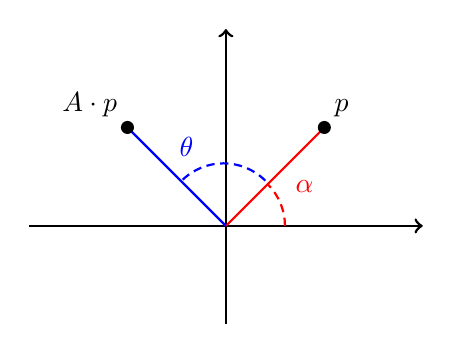
\begin{tikzpicture}[scale=2.5]
            
                    % Specifies where the x, y coordinate of the tip of
                    % the unite vectors in turn
                    \tikzset{}
            
                    % Scope used to shift the coordinates from the basis
                    \begin{scope}[shift={(0, 0, 0)}, rotate=0]
                        \coordinate (p) at (0.5, 0.5);
                        \coordinate (Ap) at (-0.5, 0.5);
                        
                    \end{scope}
            
                    % Draws the coordinate system basis with unit side lengths
                    % Is usually transparent, remove to see it for reference
                    \begin{scope}[thick, line width=1]
                        \draw[->] (-1, 0) -- (1, 0);
                        \draw[->] (0, -0.5) -- (0, 1);
                    \end{scope}
            
                    \begin{scope}[thick]
                        \draw[red] (0, 0) -- (p);
                        \draw[blue] (0, 0) -- (Ap);
                    

                        \node at (p) [circle, fill=black, scale=0.5] {};
                        \node at (p) [above right] {$p$};
                        \node at (Ap) [circle, fill=black, scale=0.5] {};
                        \node at (Ap) [above left] {$A \cdot p$};

                        \node at (0.4, 0.2) [red] {$\alpha$};
                        \node at (-0.2, 0.4) [blue] {$\theta$};
                    \end{scope}

                    \begin{scope}[thick, densely dashed]
                        % arc that begins at (x, y),
                        % from angle 1 to 2, with a raidus 
                        \draw[red] (0.3, 0) arc (0:45:0.3);
                        \draw[blue] (0.2, 0.23) arc (45:135:0.3);
                    \end{scope}      

                    \end{tikzpicture}
            
                    \caption{\label{fig:figure1} Transformation of $p$ by $A$.}
                \end{figure}
        \item 
            Proof that $\varphi: D_{2n} \to GL_2(\R)$,
            where $\varphi(r) = A$ and $\varphi(s) = B =
            \begin{pmatrix}
                0 & 1 \\
                1 & 0 \\
            \end{pmatrix}$,
            is a homomorphism: \\
            First we need to show that $B$ is the equivalent of flipping
            the $x, y$ plane around the line $y = x$.
            To do this, we must show that an arbitrary point $p$
            represented by the vector $\begin{pmatrix} x \\ y \end{pmatrix}$
            ends up on $\begin{pmatrix} y \\ x \end{pmatrix}$
            after applying the transformation
            (by multiplying the vector by matrix $B$):
            \[  \begin{pmatrix}
                0 & 1 \\
                1 & 0 \\
            \end{pmatrix} 
            \begin{pmatrix}
                x \\
                y \\
            \end{pmatrix} 
            = \begin{pmatrix}
                0 \cdot x + 1 \cdot y \\
                1 \cdot x + 0 \cdot y \\
            \end{pmatrix} 
            =  \begin{pmatrix}
                y \\
                x \\
            \end{pmatrix} \]
            So $B$'s transformation is the equivalent of a reflection 
            around the line $y = x$.
        
            % figure
            \begin{figure}[H]
            \centering
            % figure is a tikz drawing
            \begin{tikzpicture}[scale=2.5]

                % Specifies where the x, y coordinate of the tip of
                % the unite vectors in turn
                \tikzset{}
        
                % Scope used to shift the coordinates from the basis
                \begin{scope}[shift={(0, 0, 0)}, rotate=0]
                    \coordinate (p) at (0.5, 0.25);
                    \coordinate (Bp) at (0.25, 0.5);
                    
                \end{scope}
        
                % Draws the coordinate system basis with unit side lengths
                % Is usually transparent, remove to see it for reference
                \begin{scope}[thick, line width=1]
                    \draw[->] (-1, 0) -- (1, 0);
                    \draw[->] (0, -0.5) -- (0, 1);
                \end{scope}
        
                \begin{scope}[thick]
                    \node at (p) [circle, fill=black, scale=0.5] {};
                    \node at (p) [below right] {$p$};
                    \node at (Bp) [circle, fill=black, scale=0.5] {};
                    \node at (Bp) [above] {$A \cdot p$};
                    \node at (0.8, 0.8) [above right] {$f(x) = x$};
                \end{scope}

                \begin{scope}[thick, dashed]
                    \draw[red] (-0.4, -0.4) -- (0.8, 0.8);
                \end{scope}      

                \end{tikzpicture}
        
                \caption{\label{fig:figure1} Transformation of $p$ by $B$.}
            \end{figure}

            We know that $\{A, B\}$ is a set in $GL_2(\R)$,
            if its elements can be mapped to the generators of $D_{2n}$
            in such a way as to satisfy the representation's relations,
            then $\varphi$ becomes a homomorphism. \\ 
            We know that the identity matrix $I_2$ is the identity of
            $GL_2(\R)$.
            Moreover
            \[ A^n = \begin{pmatrix}
                \cos(\theta) & -\sin(\theta) \\
                \cos(\theta) & \sin(\theta) \\
            \end{pmatrix}^n
            = \begin{pmatrix}
                \cos(n \cdot \theta) & -\sin(n \cdot \theta) \\
                \cos(n \cdot \theta) & \sin(n \cdot \theta) \\
            \end{pmatrix} \]
            \[ = \begin{pmatrix}
                \cos(\sfrac{2n \pi}{n}) & -\sin(\sfrac{2n \pi}{n}) \\
                \cos(\sfrac{2n \pi}{n}) & \sin(\sfrac{2n \pi}{n}) \\
            \end{pmatrix} 
             = \begin{pmatrix}
                \cos(2\pi) & -\sin(2\pi) \\
                \cos(2\pi) & \sin(2\pi) \\
            \end{pmatrix}
            = \begin{pmatrix}
                1 & 0 \\
                0 & 1 \\
            \end{pmatrix} = I_2 \]
            and
            \[ B^2 = \begin{pmatrix}
                0 & 1 \\
                1 & 0 \\
            \end{pmatrix}^2 
            =  \begin{pmatrix}
                1 & 0 \\
                0 & 1 \\
            \end{pmatrix} = I_2 \] 
            and we have
            \[ AB = \begin{pmatrix}
                \cos(\theta) & -\sin(\theta) \\
                \cos(\theta) & \sin(\theta) \\
            \end{pmatrix}
            \begin{pmatrix}
                1 & 0 \\
                0 & 1 \\
            \end{pmatrix}
            = \begin{pmatrix}
                -\sin(\theta) & \cos(\theta) \\
                \cos(\theta) & \sin(\theta) \\
            \end{pmatrix} \]
            which in turn, is equal to
            \[ BA^{-1} = \begin{pmatrix}
                1 & 0 \\
                0 & 1 \\
            \end{pmatrix}
            \begin{pmatrix}
                \cos(\theta) & -\sin(\theta) \\
                \cos(\theta) & \sin(\theta) \\
            \end{pmatrix}^{-1}
            =  \begin{pmatrix}
                1 & 0 \\
                0 & 1 \\
            \end{pmatrix}
            \dfrac{\begin{pmatrix}
                -\sin(\theta) & \cos(\theta) \\
                \cos(\theta) & \sin(\theta) \\
            \end{pmatrix}}{\cos^2(\theta) + \sin^2(\theta)} \]
            \[ = \begin{pmatrix}
                1 & 0 \\
                0 & 1 \\
            \end{pmatrix}
            \dfrac{\begin{pmatrix}
                \cos(\theta) & \sin(\theta) \\
                -\sin(\theta) & \cos(\theta) \\
            \end{pmatrix}}{1} 
            = \begin{pmatrix}
                -\sin(\theta) & \cos(\theta) \\
                \cos(\theta) & \sin(\theta) \\
            \end{pmatrix} = AB \]
            So the relations are satisfied,
            but since $A$ and $B$ are not $GL_2(\R)$'s generators,
            $\varphi$ is a non-surjective homomorphism.
        \item
            Proof that $\varphi$ is injective: \\
            By exercise 1.1.6.13,
            we know that $\varphi(D_{2n}) \leqslant GL_2(\R)$.
            This subrgoup is generated by $A$ and $B$.
            Since we have $A^n = B^2 = 1$,
            and $AB = BA^{-1}$,
            we can conclude (as we have done before)
            that the elements in $\varphi(D_{2n})$
            are of the form $A^n$ or $BA^n$.
            So we have $2 \times n$ different combinations.
            Which means that $|\varphi(D_2n)| = 2n = |D_{2n}|$.
            Since $\varphi$ is well defined,
            that means that each element in $D_{2n}$ maps to exactly
            one element in $GL_2(\R)$.
            So $\varphi$ is injective.
    \end{enumerate}

    
    \section*{Exercise 26}
    Proof that $\varphi: Q_8 \to GL_2(\C)$ defined by
    \[  \varphi(i) = A =\begin{pmatrix}
        \sqrt{-1} & 0 \\
        0 & \sqrt{-1} \\
    \end{pmatrix}
    \quad \text{and} \quad
    \varphi(j) = B =\begin{pmatrix}
        0 & -1 \\
        1 & 0 \\
    \end{pmatrix} \]
    extends to a homomorphism: \\
    In 1.1.5.3, we showed that
    \[  Q_8 = \langle i, j \mid i^2 = j^2, i^4 = 1, i = jij \rangle \]
    Moreover, we have
    \[  A^2 = \begin{pmatrix}
        \sqrt{-1} & 0 \\
        0 & \sqrt{-1} \\
    \end{pmatrix}^2
    = \begin{pmatrix}
        (\sqrt{-1})^2 & 0 \\
        0 & (\sqrt{-1})^2 \\
    \end{pmatrix}
    = \begin{pmatrix}
        -1 & 0 \\
        0 & -1 \\
    \end{pmatrix} \]
    which is equal to
    \[  B^2 = \begin{pmatrix}
        0 & -1 \\
        1 & 0 \\
    \end{pmatrix}^2
    = \begin{pmatrix}
        -1 & 0 \\
        0 & -1 \\
    \end{pmatrix} = A^2 \]
    Furthermore
    \[  A^4 = (A^2)^2 = \begin{pmatrix}
        -1 & 0 \\
        0 & -1 \\
    \end{pmatrix}^2
    = \begin{pmatrix}
        (-1)^2 & 0 \\
        0 & (-1)^2 \\
    \end{pmatrix}
    = \begin{pmatrix}
        1 & 0 \\
        0 & 1 \\
    \end{pmatrix} = I_2 \]
    where $I_2$ is the identity matrix,
    and the identity of $GL_2(\C)$. \\
    And finally
    \[  BAB = \begin{pmatrix}
        0 & -1 \\
        1 & 0 \\
    \end{pmatrix}
    \begin{pmatrix}
        \sqrt{-1} & 0 \\
        0 & \sqrt{-1} \\
    \end{pmatrix}
    \begin{pmatrix}
        0 & -1 \\
        1 & 0 \\
    \end{pmatrix} \]
    \[ = \begin{pmatrix}
        0 & \sqrt{-1} \\
        \sqrt{-1} & 0 \\
    \end{pmatrix}
    \begin{pmatrix}
        0 & -1 \\
        1 & 0 \\
    \end{pmatrix}
    = \begin{pmatrix}
        \sqrt{-1} & 0 \\
        0 & \sqrt{-1} \\
    \end{pmatrix} = A \]
    Since $A$ and $B$ are in $GL_2(\C)$,
    and since mapping $i$ and $j$, $Q_8$'s generators, to them
    satisfied $Q_8$'s relations,
    that makes the mapping $\varphi$ a homomorphism
    (non-surjective as $A$ and $B$ don't generate $GL_2(\C)$). \\
    Proof that $\varphi$ is injective:
    By 1.1.6.13, we know that $\varphi(Q_8) \leqslant GL_2(\C)$.
    We know that $A$ and $B$ generate $\varphi(Q_8)$,
    so $\varphi(Q_8) = \{ 1, -1, A, B, A^{-1}, B^{-1}, AB, BA \}$.
    (any other combination produces one of the elements in the set).
    So $|\varphi(Q_8)| = 8 = Q_8$.
    Hence, as $\varphi$ is well defined, each element in $Q_8$
    maps to exactly one element in $GL_2(\C)$,
    making the mapping injective.
        
\end{document}
